\chapter{Implemented Solution}
\section{Amazon Web Services}

\subsection{Architecture}
\begin{figure}[h]
    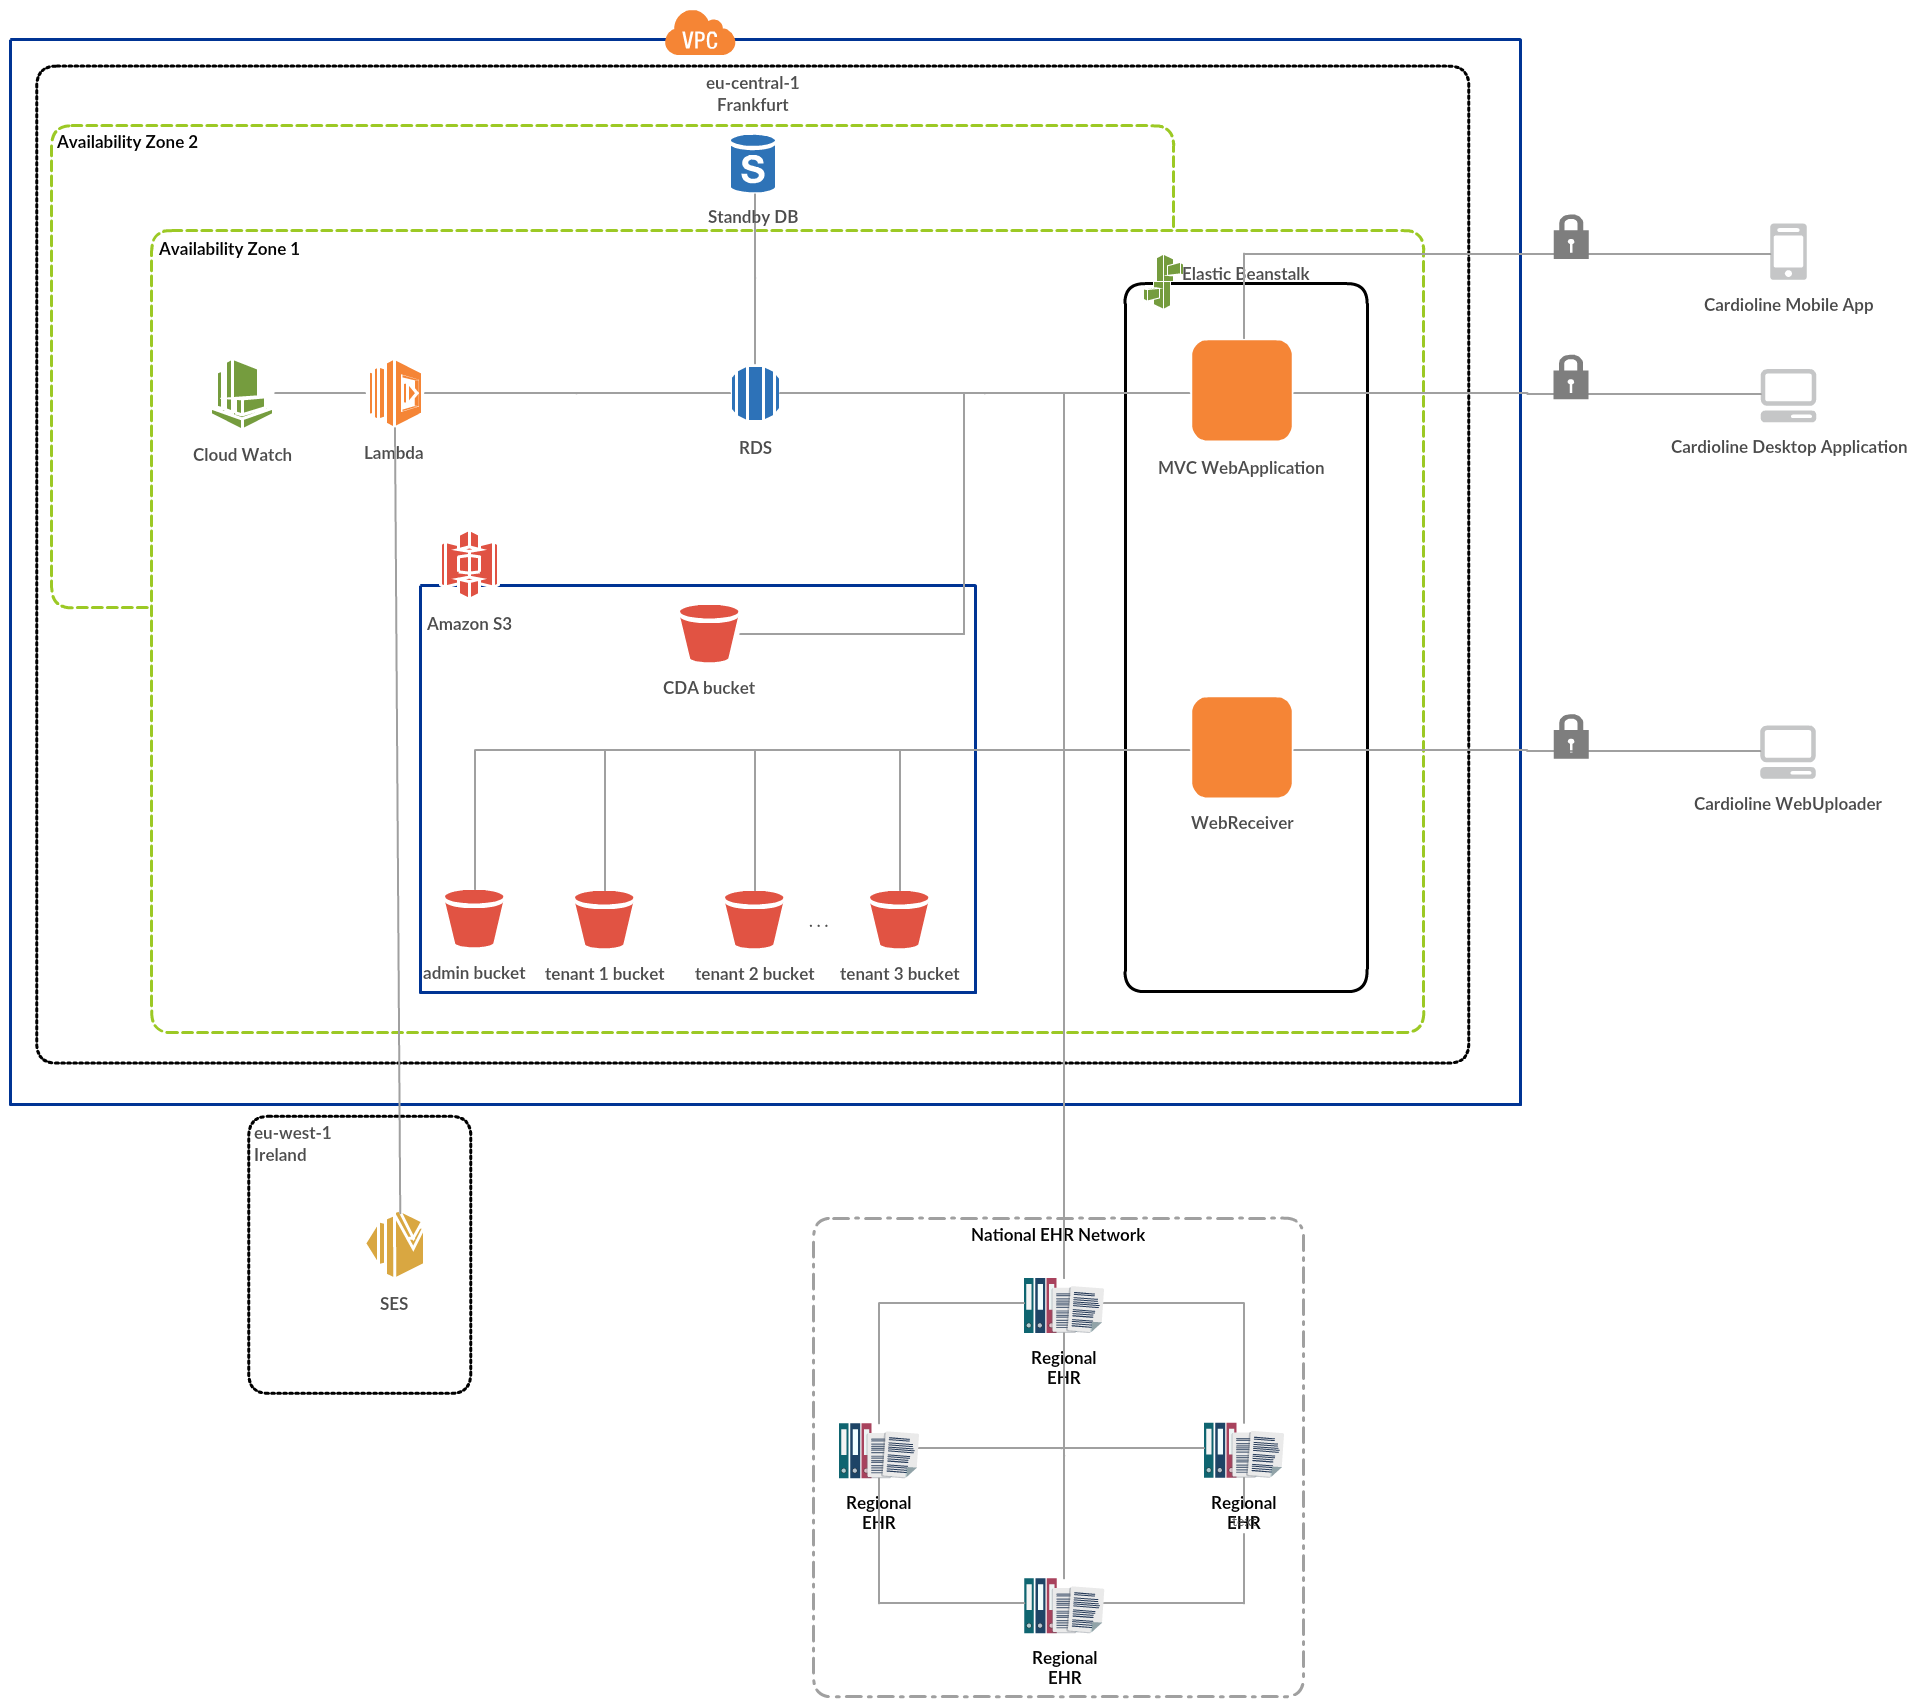
\includegraphics[width=\textwidth]{img/architecture}
    \caption{Architecture Scheme}
    \label{fig:architecture}
\end{figure}
Since Amazon Elastic Beanstalk (EB) has been used as the core component of the system, it has been possible to use an infrastructure as a service (IaaS \ref{paragraph:Iaas}) grade of customization, with an easier configuration and building phase as if the system was platform as a service (PaaS \ref{paragraph:Paas}) instead.\\
As shown in picture \ref{fig:architecture}, everything but the Amazon Simple Email Service (SES \cite{AmazonSes}) service is hosted in the eu-central-1 region in Frankfurt to reduce latency, minimize costs and keep healthcare data in an European law venue, as in production would be.
The region is divided into availability zones connected to each other with low-latency links, so to handle potential instance failures by replacing them with the standby ones located in a different availability zone.\\
EB handles the WebServer instances: one for the EcgWebApp, more details in section \ref{subsection:ecgwebapp} and the other one for WebReceiver,section \ref{subsection:webreceiver}. The interaction is then allowed to authenticated users bounded to their capabilities and role.\\
The persistency is achieved by a Relational Database Service (RDS) running Amazon Aurora DB, a compatible MySql Database organized with a master write replica and several read replicas.
Furthermore, RDS provides a standby and synchronous Database, hosted in another availability zone, that is ready to become the new master in case of failure of the current master.\\
All the assets and static files are read and written from/to AWS S3 relative bucket.\\
The notification System is triggered by DB events and carried on by AWS Lambda functions using Amazon Simple Email Service (SES) as delivery service to final users. This service is not available in the Frankfurt region hence, the Ireland region was chosen.


\section{Ecg Workflow}

%\begin{figure}[h]
%    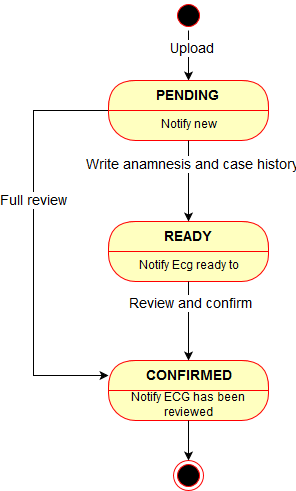
\includegraphics[width=5cm]{img/ECGstatechart}
%    \caption{Electrocardiogram State Chart}
%    \label{fig:ECGstatechart}
%\end{figure}

\begin{wrapfigure}{r}{8cm} %this figure will be at the right
    \centering
    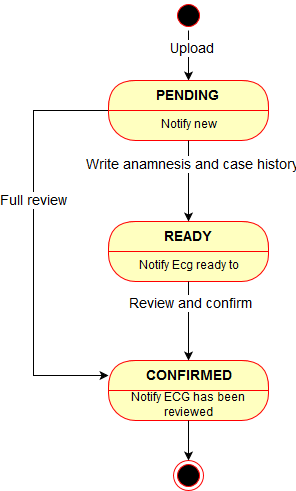
\includegraphics[width=8cm]{img/ECGstatechart}
    \caption{Electrocardiogram State Chart}
    \label{fig:ECGstatechart}
\end{wrapfigure}
 

Resting Electrocardiogram (\ref{paragraph:Resting}) are uploaded from different device types such as, mobile phones, desktop computers and Cardioline specific machines to EcgWebApp through a specific REST (\ref{paragraph:REST}) interface, the exam is stored in a \textit{pending} state and every associated referring physician notified.
Once a \textit{pending} exam is reported
\section{Web Applications Involved}
\subsection{EcgWebApp}
\label{subsection:ecgwebapp}
\subsection{Web Receiver}
\label{subsection:webreceiver}
\subsection{Web Uploader}
\section{S3 Bucket synchronization}
\section{Interoperability of digital electrocardiograms data}
\paragraph{Resting}
\label{paragraph:Resting}
\paragraph{Cardiac stress test}
\label{paragraph:Cardiac stress test}
\paragraph{Holter}
\label{paragraph:Holter}




